\documentclass{article}


\usepackage{arxiv}

\usepackage[utf8]{inputenc} % allow utf-8 input
\usepackage[T1]{fontenc}    % use 8-bit T1 fonts
\usepackage{hyperref}       % hyperlinks
\usepackage{url}            % simple URL typesetting
\usepackage{booktabs}       % professional-quality tables
\usepackage{amsfonts}       % blackboard math symbols
\usepackage{nicefrac}       % compact symbols for 1/2, etc.
\usepackage{microtype}      % microtypography
\usepackage{lipsum}
\usepackage{graphicx}
\usepackage{float}
\usepackage{subcaption}
\graphicspath{ {./figures/} }

\title{Multilayer Summary}


\author{
Jiarong Wu
%   David S.~Hippocampus\thanks{Use footnote for providing further
%     information about author (webpage, alternative
%     address)---\emph{not} for acknowledging funding agencies.} \\
%   Department of Computer Science\\
%   Cranberry-Lemon University\\
%   Pittsburgh, PA 15213 \\
%   \texttt{hippo@cs.cranberry-lemon.edu} \\
  %% examples of more authors
   \And
Luc Deike
}

\begin{document}
\maketitle

% \begin{abstract}
% \lipsum[1]
% \end{abstract}

% keywords can be removed
% \keywords{First keyword \and Second keyword \and More}
\section{Introduction to multilayer solver}

\section{Test case set 1: Stokes wave in 1m box}
\subsection{Non-breaking case}
Slope $ak = 0.1$. With viscosity $\nu = 1/40,000$, wave number $k = 2\pi$, this gives a theoretical dissipation rate $a = -4\nu k^2 = -0.0063$. The dissipation rate extracted from the energy curve is surprisingly even smaller than that, with a small difference between the two horizontal resolution cases.
\begin{figure}[H]
    \begin{subfigure}{0.5\linewidth}
    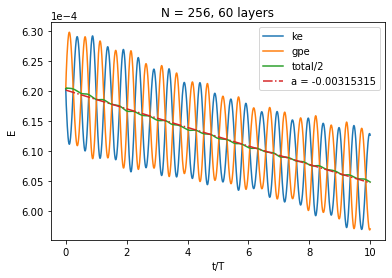
\includegraphics[width=\linewidth]{figures/stokes_ak01_256.png} 
    \end{subfigure}
    \begin{subfigure}{0.5\linewidth}
    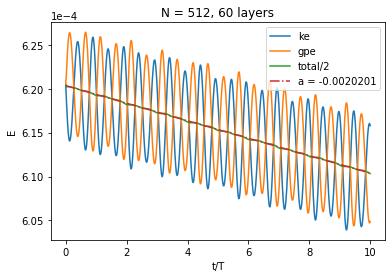
\includegraphics[width=\linewidth]{figures/stokes_ak01_512.png}
    \end{subfigure}
    \caption{Left: exponential with horizontal resolution 256. Right: exponential with horizontal 512. Both 60 layers.}
    \label{fig:fig1}
\end{figure}
\begin{figure}[H]
    \begin{subfigure}{0.5\linewidth}
    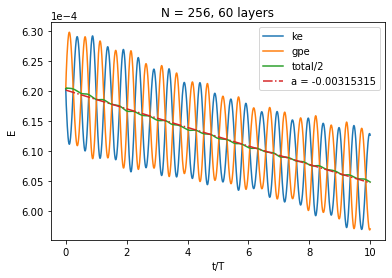
\includegraphics[width=\linewidth]{figures/stokes_ak01_256.png} 
    \end{subfigure}
    \begin{subfigure}{0.5\linewidth}
    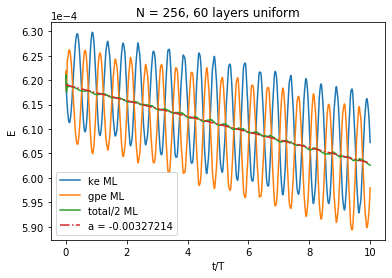
\includegraphics[width=\linewidth]{figures/stokes_ak01_256_uniform.png}
    \end{subfigure}
    \caption{Left: exponential grid. Right: uniform grid. No apparent effect on the dissipation rate.}
    \label{fig:fig1}
\end{figure}

\subsection{Breaking case and comparison with DNS}
\begin{figure}[h!]
    \centering
    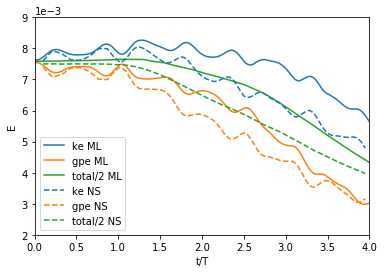
\includegraphics[width=0.8\linewidth]{figures/stoke_mlns_comparison.png}
    \caption{ML and NS stands for multilayer and DNS solver respectively. Grid configuration for the ML case is 60 layers UNIFORM grid, 256*256 horizontally.}
    \label{fig:fig1}
\end{figure}

In this case, using exponential grid with the same layer number GREATLY affects the breaking happening point. Which needs some further investigation.

\begin{figure}[H]
    \begin{subfigure}{0.5\linewidth}
    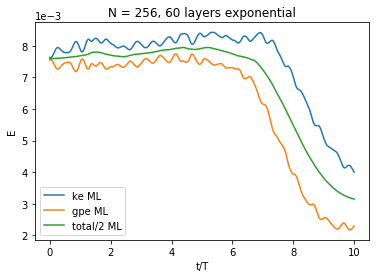
\includegraphics[width=\linewidth]{figures/stokes_ak035_256.png} 
    \end{subfigure}
    \begin{subfigure}{0.5\linewidth}
    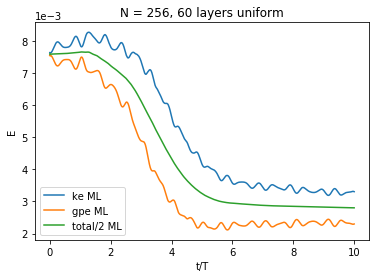
\includegraphics[width=\linewidth]{figures/stokes_ak035_256_uniform.png}
    \end{subfigure}
    \caption{Left: exponential grid. Right: uniform grid. Big difference in breaking point.}
    \label{fig:fig1}
\end{figure}

A snapshot comparison of ML and NS. Still needs to tweak the camera angle and size. Maybe also run for longer time.
COLORBAR.
\begin{figure}[H]
    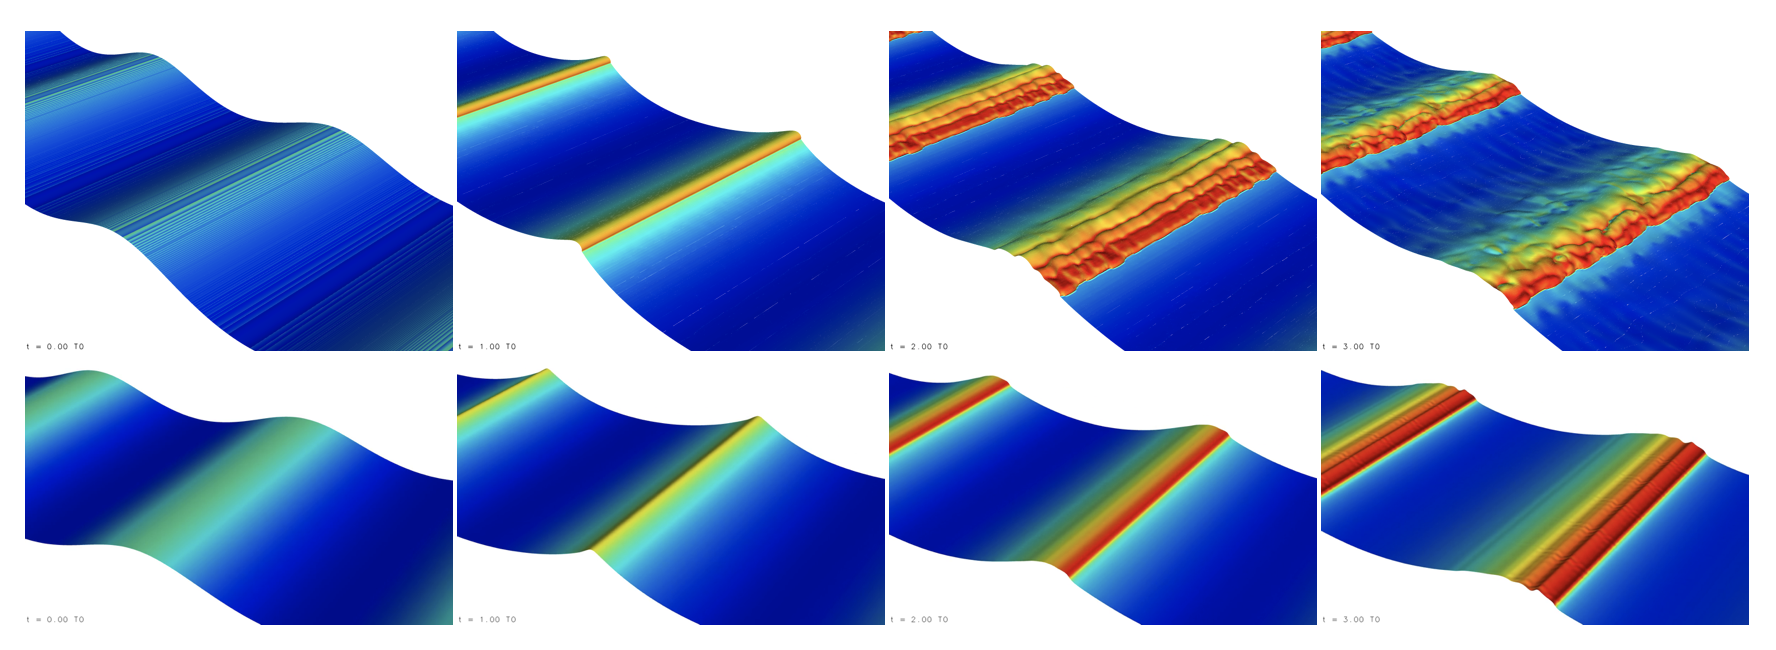
\includegraphics[width=\linewidth]{figures/stokes_snapshot.png} 
    \caption{Top row: Navier-Stokes solver (NS). Bottom row: multilayer solver (ML). Color denotes horizontal velocity.}
    \label{fig:fig1}
\end{figure}

\section{Test case set 2: Field scale controlled tests}

Short crested focusing wave
series of snapshot
plot of energy
extract length of crest
axis to the plot
Both surface elevation and slope

Videos of random breaking and energy curve

Initial spectrum.

With the exponential configuration we have seen a delay in breaking

\subsection{Train of 5 waves, non breaking}
Train of 5 waves of $k_p=2\pi/10$ rad/m. $ak=0.1$. $\nu=1/40,000$. It seems with the good horizontal/vertical setup we have reasonable limited viscous decay. Run long time (like 100 wave period) to see if the decay is ok.

\subsection{Focusing unidirectional wave train, breaking}
Peak wave number $k_p=2\pi/10$ rad/m. $\nu=1/40,000$. Spatial 2d focusing of breaking wave using the same config as for the 1D test. See how it looks. Compute the turbulent dissipation rate $\epsilon_l$ as in experimental paper/numerical paper. Compute the breaking parameter $b$. See if it falls in the master curve $b=0.4(S-0.08)^{5/2}$
\section{Random wave field}
The spectrum used to initialize the wave field is given by 
\begin{equation}
    F(k) = Pk^{-2.5}exp[-0.75*(k_p/k)^2]
\end{equation}
Peak wave number $k_p=2\pi/10$ rad/m. Select three amplitudes. Define $a^2 = \overline{\eta^2}$. Then work with $ak_p$ = 0.05, 0.1, 0.15.

\subsection{500m box}




\bibliographystyle{unsrt}  
%\bibliography{references}  %%% Remove comment to use the external .bib file (using bibtex).
%%% and comment out the ``thebibliography'' section.
%%% Comment out this section when you \bibliography{references} is enabled.
\begin{thebibliography}{1}
\end{thebibliography}

\end{document}
